\clearpage
\vspace*{\stretch{2}}%{\fill}
\begin{center}
\begin{minipage}{.75\textwidth}
\section{Tecnologías utilizadas}

Para el correcto funcionamiento de nuestro sistema de sensado móvil colaborativo asimétrico con beneficios dispares es necesario el uso del hardware básico presentado en el capítulo 2 y de un conjunto de aplicaciones software. En este capítulo presentamos una descripción somera de todas las tecnologías utilizadas para el desarrollo del proyecto. % \pagebreak
\end{minipage}
\end{center}
\vspace{\stretch{3}} % \vfill % equivalent to \vspace{\fill}
\clearpage% https://tex.stackexchange.com/questions/70714/center-horizontally-and-vertically-a-block-of-text

\subsection{Introducción}
Como habíamos comentado en el capítulo 2, el \emph{hardware} que necesita el propietario del local es básicamente una Rapberry Pi 3. Para que el sistema de sensado funcione debemos instalar en la Raspberry Pi 3 \emph{software} que nos permita definir la funcionalidad del portal cautivo que nos permitiría implantar la aplicación de sensado móvil colaborativo de acceso a Internet. En la Figura \ref{CoovaScheme} se muestra un esquema general del \emph{software} necesario. En concreto instalamos el siguiente:

\begin{figure}[!t]
\begin{center}
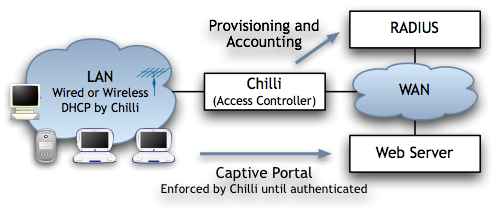
\includegraphics[width=0.75\linewidth]{./3_Tecnologias/Img/CoovaScheme.jpg}
\end{center}
\caption{Esquema general del Software utilizado para la implantación del portal cautivo}
\source{http://coova.github.io/CoovaChilli/}
\label{CoovaScheme}
\end{figure}

\begin{itemize}
\item \emph{Host Access Point Daemon} (\emph{\acrshort{Hostapd}}) \cite{hostapdDoc}: este daemon de linux se encarga de configurar el módulo WiFi en modo \acrshort{AP}. De esta manera, la Raspberry Pi 3 puede actuar como un punto de acceso configurable, conectándose sus clientes a través de su interfaz \acrshort{WiFi} y obteniendo acceso a la red a través de la interfaz Ethernet de acuerdo al esquema que se muestra en la Figura 2.3.
\item \emph{CoovaChilli} \cite{ChilliGitHub}: el software controlador de acceso que proporcionaría direcciones \emph{Internet Protocol} (\acrshort{IP}) a las conexiones entrantes con su \emph{Dynamic Host Control Protocol} (\acrshort{DHCP}), redirigiría dichas conexiones al portal cautivo para su autenticación en el sistema y las gestionaría junto a un sistema de Autenticación, Autorización y Contabilización (\acrshort{AAA}) que ha de ser instalado aparte, habitualmente un servidor \emph{Remote Authentication Dial-In User Service} (\acrshort{RADIUS}) \cite{RADIUS}.
\item \emph{FreeRADIUS} \cite{FreeRADIUSDoc}: el servicio de \acrshort{AAA} gracias al cual CoovaChilli controla los usuarios del sistema. Para su utilización es necesaria su previa integración con My\acrshort{SQL} \cite{PHPMySQLJavaScript}, que ha de estar instalado en el sistema.
\item \emph{daloRADIUS} \cite{daloRADIUS1}: plataforma Web destinada a controlar el servidor RADIUS de forma gráfica. En este TFG, su contenido es proporcionado por un servidor web.
\item \emph{Node.js}: tecnología JavaScript (para el servidor), complementada con paquetes \acrshort{npm}, con la que implantamos el back-end de nuestra aplicación Web de portal cautivo, que interactuaría con CoovaChilli por medio de su interfaz \acrshort{JSON}.
\item \emph{Front end Web}: página Web a la que acceden los clientes a través de su teléfono móvil implantada en Node.js a partir de: \acrshort{HTML}, \acrshort{CSS} y JavaScript. Esta página Web es el principal elemento diferenciador respecto a otros portales cautivos habituales, dado que su propósito sería el de recopilar del usuario, a través de su navegador, los datos del micrófono del dispositivo conectado al portal cautivo a través de su navegador. Esto es posible gracias a la \emph{Application Programming Interface} (\acrshort{API}) \emph{MediaStream Recording} \cite{MediaStreamRecordingAPI}, tecnología estrechamente relacionada con \emph{\acrshort{WebRTC}} \cite{LibroWebRTC1}.
\end{itemize}

A continuación se realiza un análisis más pormenorizado de las tecnologías utilizadas. Se considera que el lector tiene un conocimiento al menos elemental de las tecnologías Web tradicionales, por lo que estas solo se introducen de forma superficial exceptuando aquellos aspectos concretos que tienen relevancia en este TFG. Los elementos \emph{software} más específicos reciben un análisis pormenorizado, entrando en mayores detalles.

\subsection{\emph{Software} necesario para el funcionamiento básico de la Raspberry Pi 3}
La Raspberry Pi es un tipo de sistema empotrado de pequeño tamaño. Es un computador de un sola placa madre, de reducidas dimensiones. Inicialmente fue planteado como un dispositivo de bajo coste (35 \$) y consumo energético (1.5 W) en su último modelo. Está orientado a propósitos educativos en colegios y países en vías de desarrollo, aunque su uso se extendió rápidamente a otros ámbitos como la robótica. Sus modelos son desarrollados por la Raspberry Pi Foundation en el Reino Unido y actualmente se le considera el ordenador de esa región más vendido.

Desde su introducción en Febrero de 2012 ha habido varias generaciones de este dispositivo, siendo la más reciente la Raspberry Pi 3 Model B que es la usada en este TFG. Este modelo consta de un \emph{Sistema en Chip} (\acrshort{SoC}) de Broadcom, que incluye un procesador quad-core compatible con -\acrshort{ARM}v8 de 64 bits que opera a una frecuencia de 1.2 GHz y un procesador gráfico. Cuenta también con 1GB de \emph{Random Access Memory} (\acrshort{RAM}) \acrshort{LPDDR2} a 900 MHz. Para almacenar el sistema operativo se utiliza una tarjeta \acrshort{MicroSDHC}, y aunque puede instalarse una gran variedad de sistemas operativos diferentes el recomendado es Linux basado en Debian (renombrado como \emph{Raspbian}). En cuanto a entrada-salida la Raspberry Pi 3 cuenta con cuatro puertos \emph{Universal Serial Bus} (\acrshort{USB}), interfaz Ethernet 10/100 Mbps y salidas \emph{High-Definition Multimedia Interface} (\acrshort{HDMI}) y minijack de audio. También incorpora 40 pines entrada-salida de propósito general (\emph{\acrshort{GPIO}, General Purpose Input-Output}) para operaciones a bajo nivel. Otro aspecto de importancia crucial para este TFG es la conectividad inalámbrica, dado que la Raspberry Pi 3 incorpora chipsets \acrshort{WiFi} (versión \acrshort{IEEE} 802.11n) para 2.4 GHz a 150 Mbps y Bluetooth 4.1 a 24 Mbps. Además de esto, en la actualidad se fabrica una amplia gama de accesorios destinados a ampliar la funcionalidad de la Raspberry Pi como cámaras de vídeo, interfaces de control de \acrshort{LED}s y sensores y otras placas de expansión.

\subsubsection{Raspbian y WiFi}

El Raspbian es el sistema operativo recomendado por la Raspberry Pi Foundation desde 2015. Está basado en Debian Jessie y fue desarrollado por Mike Thompson y Peter Green poniendo especial énfasis en los procesadores \acrshort{ARM} de bajo rendimiento de la Raspberry Pi. Incluyen Python, Scratch, Java, Sonic Pi, Mathematica entre otros programas relevantes.

Utiliza \emph{Pi Improved Xwindows Environment Lightweight} (\acrshort{PIXEL}) como entorno gráfico de escritorio. Consiste en un entorno de escritorio \emph{Lightweight X11 Desktop Environment} (\acrshort{LXDE}) modificado y el gestor de ventanas Openbox.
La principal característica de la Raspberry Pi 3 para este TFG es su capacidad de manejo de la tecnología WiFi. Esta tecnología especifica el nivel físico y el subnivel de control de acceso al medio (\acrshort{MAC}, \emph{Medium Access Control}). La versión con la que se ha trabajado es la \acrshort{IEEE} 802.11n, que soporta el uso de varias antenas simultáneamente (\emph{\acrshort{MIMO}, Multiple Input Multiple Output}), aprovechando la propagación multitrayecto para aumentar la tasa de transferencia, e incorpora mejoras en seguridad, agregación de trama, técnicas de \emph{beamforming} para optimizar la emisión de señal junto a otros aspectos. Aunque \acrshort{IEEE} 802.11n también permite trabajar en la frecuencia de 5 GHz, el dispositivo que hemos utilizado como punto de acceso \acrshort{WiFi} trabajaba en 2.4 GHz.

\subsubsection{Hostapd}

Es una utilidad software cuya funcionalidad es transformar las interfaces de red en puntos de acceso y servidores de autenticación. Implementa la gestión de puntos de acceso \acrshort{IEEE} 802.11, autenticación \acrshort{IEEE} 802.11X, \emph{\acrshort{WiFi} Protected Access} (WPA), \acrshort{WPA2}, \emph{Extensible Authentication Protocol} (\acrshort{EAP}), cliente \acrshort{RADIUS}, servidor \acrshort{EAP} y servidor de autenticación \acrshort{RADIUS}. Soporta interfaces con drivers presentes en sistemas Linux y FreeBSD.

Como \emph{daemon} ha sido diseñado para operar en segundo plano como componente \emph{back-end}, soportando aplicaciones front-end separadas. Ha sido programado para funcionar de forma modular por medio de código C organizado en archivos separados. En la Figura \ref{hostapd} se muestra un esquema de la organización del funcionamiento de \acrshort{Hostapd}.

\begin{figure}[!t]
\begin{center}
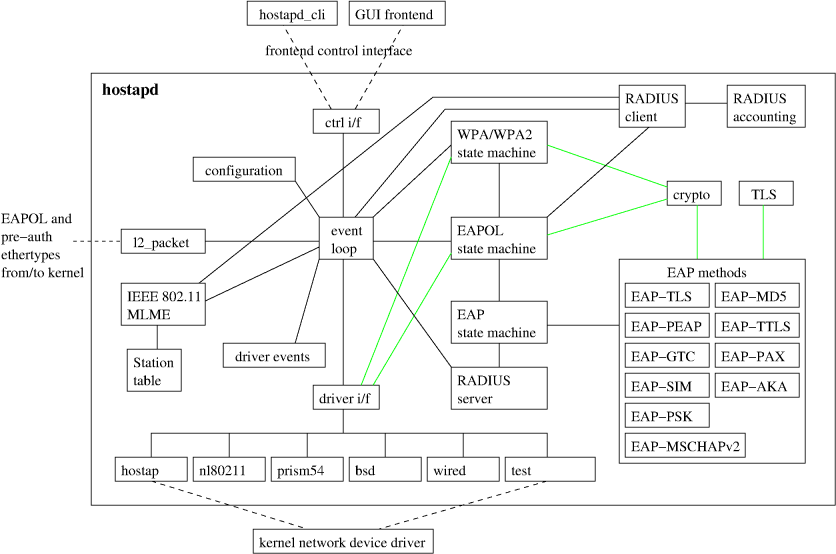
\includegraphics[width=0.75\linewidth]{./3_Tecnologias/Img/hostapd.png}
\end{center}
\caption{Esquema general del funcionamiento de Hostapd}
\source{http://w1.fi/wpa\_supplicant/devel/}
\label{hostapd}
\end{figure}

Hostapd se configura por medio de un archivo de texto que lista todos los parámetros de configuración, alojado en el archivo \emph{/etc/hostapd/hostapd.conf}, que cuenta con los siguientes atributos relevantes y comúnmente utilizados, entre otros:
\begin{itemize}
\item Atributos de Interfaz Inalámbrica:
\begin{itemize}
\item \emph{interface}: interfaz inalámbrica va a utilizarse.
\item \emph{bridge}: interfaz puente si la interfaz inalámbrica es parte de ella.
\item \emph{driver} (controlador utilizado): suele ser n18011.
\end{itemize}
\item Atributos de Entorno Inalámbrico:
\begin{itemize}
\item \emph{ssid}: nombre o \emph{Service Set IDentifier} (\acrshort{SSID}) de la red que aparecería en la lista de redes disponibles al hacer la habitual búsqueda de red desde un dispositivo inalámbrico.
\item \emph{hw\_mode}: fija el modo de operación de la interfaz y los canales permitidos. Los valores permitidos dependen del hardware pero siempre son un subconjunto de \emph{a}, \emph{b} o \emph{g}. Aunque se configure una red \acrshort{IEEE} 802.11n no es aquí donde debe indicarse, ya que \acrshort{IEEE} 802.11n opera sobre la funcionalidad de \acrshort{IEEE} 802.11a o \acrshort{IEEE} 802.11g.
\item \emph{channel}: el canal en el que Hostapd operaría como punto de acceso. Debe ser un canal soportado por el modo de hardware establecido en el atributo \emph{hw\_mode}. Los canales de \acrshort{IEEE} 802.11 son de 20 MHz de anchura (4 canales) en el espectro, solapándose entre ellos, por lo que deben escogerse de forma que esto no suceda. Por ejemplo, si la mayoría de puntos de acceso de la red utilizan el canal 6 sería óptimo utilizar el canal 1 o el canal 11 para evitar interferencias por solapamiento.
\end{itemize}
\item Atributos de \acrshort{IEEE} 802.11n:
\begin{itemize}
\item \emph{ieee80211n}: atributo booleano que al asignársele el valor 1 activa las funcionalidades propias de \acrshort{IEEE} 802.11n.
\item \emph{ht\_capab}: lista de las capacidades \acrshort{IEEE} 802.11n soportadas por el dispositivo utilizado. Actúan como flags, activándose al ser escritos entre corchetes. Ejemplos de ello serían habilitar el uso de canales de 40 MHz (\emph{[HT40+]}) o activar el modo \acrshort{DSSS}/\acrshort{CCK} en dichos canales (\emph{[DSSS\_CCK-40]}).
\end{itemize}
\item Autenticación y cifrado:
\begin{itemize}
\item \emph{macaddr\_acl}: controla el filtrado de direcciones \acrshort{MAC}.
\item \emph{auth\_algs}: campo de bits en el que el primero es para autenticación abierta, el segundo es por autenticación de Clave Compartida (\acrshort{WEP}), pudiendo activar ambos introduciendo un 3.
\item \emph{ignore\_broadcast\_ssid}: activa o desactiva la difusión del \acrshort{SSID}.
\item \emph{wpa}: Un campo de bits como \emph{auth\_algs}. El primero activa \acrshort{WPA}1, el segundo activa \acrshort{WPA2} y el 3 activa los dos.
\item \emph{wpa\_psk} o \emph{wpa\_passphrase}: contraseña para la autenticación \acrshort{WPA}.
\item \emph{wpa\_key\_mgmt}: controla con qué algoritmos de gestión de claves podría autenticarse un cliente.
\item \emph{wpa\_pairwise}: controla el encriptado de datos de \acrshort{WPA}.
\item \emph{rsn\_pairwise}: controla el encriptado de datos de \acrshort{WPA2}.
\end{itemize}
\end{itemize}

En el bloque de código \ref{HostapdConf1} se muestra un ejemplo de archivo de configuración. 

\begin{listing}[H]
\begin{minted}
[
frame=lines,
framesep=2mm,
baselinestretch=1.2,
bgcolor=lightgray,
fontsize=\footnotesize,
breaklines=true,
breaksymbolleft={}
]
{bash}
interface=wlan0
driver=nl80211
ssid=RaspAP
hw_mode=g
channel=8
wpa=2
wpa_psk=928519398acf811e96f5dcac68a11d6aa876140599be3dd49612e760a2aaac0e
wpa_key_mgmt=WPA-PSK
wpa_pairwise=CCMP
rsn_pairwise=CCMP
beacon_int=100
auth_algs=3
wmm_enabled=1
\end{minted}
\caption{Ejemplo de archivo de configuración de Hostapd}
\label{HostapdConf1}
\end{listing}

\subsection{El Servidor RADIUS}

CoovaChilli hace uso de servicios de \acrshort{AAA} separados para poder funcionar. Habitualmente este servicio es un servidor \acrshort{RADIUS} instalado de forma separada. Por ello, se exponen algunos detalles de su funcionamiento, junto a detalles la solución concreta de servidor \acrshort{RADIUS} utilizada en este TFG, FreeRADIUS, y otros aspectos relevantes.

RADIUS es un protocolo cliente/servidor que proporciona gestión de AAA de forma centralizada para aquellos clientes de un servicio de Red. Fue desarrollado en 1991 por parte de Livingston Enterprises, Inc. como un protocolo de autenticación y contabilidad para servidores de acceso, convirtiéndose en un estándar de la \emph{Internet Engineering Task Force} (\acrshort{IETF}). Se implanta a nivel de aplicación y puede utilizar tanto \emph{Transmission Control Protocol} (\acrshort{TCP}) como \emph{User Datagram Protocol} (\acrshort{UDP}). \acrshort{RADIUS} suele ser el back-end para autenticaciones de \acrshort{IEEE} 802.11x, como un proceso en segundo plano ejecutándose en un servidor UNIX o Windows. Actualmente se utiliza de forma prácticamente masiva por proveedores de servicios de Internet para gestionar el acceso al mismo o a redes internas, inalámbricas y a servicios de correo electrónico.

\subsubsection{El Servidor RADIUS}

La autenticación y autorización de RADIUS es la descrita en la \emph{Request For Comments} (\acrshort{RFC}) 2865 mientras que la contabilidad es la descrita en la \acrshort{RFC} 2866.

Para la autenticación y autorización, el cliente envía una petición al \emph{Servidor de Acceso a la Red} (\acrshort{NAS}) para obtener acceso a un recurso de red particular utilizando credenciales de acceso. Estas credenciales llegan a este dispositivo mediante los protocolos de nivel de enlace. En respuesta, el \acrshort{NAS} envía un mensaje RADIUS de Petición de Acceso al servidor RADIUS, pidiendo autorización para conceder el acceso mediante el protocolo \acrshort{RADIUS}. Esta petición incluye credenciales de acceso, habitualmente un nombre de usuario y contraseña o un certificado de seguridad proporcionados por el usuario. El servidor RADIUS comprueba que la información es correcta utilizando patrones de autenticación como \emph{Password Authentication Protocol} (\acrshort{PAP}), \emph{Challenge-Handshake Authentication Protocol} (\acrshort{CHAP}) o \acrshort{EAP}. En este punto se verifica la información de identificación con las almacenadas en un archivo del servidor o una fuente externa, como una base de datos \acrshort{SQL}. Tras esto, el servidor \acrshort{RADIUS} puede responder de tres formas (Figura \ref{RADIUSAccept}):

\begin{itemize}
\item \emph{Access Accept}: se concede acceso al usuario.
\item \emph{Access Challenge}: solicita información adicional, como una contraseña secundaria o un PIN.
\item \emph{Access Reject}: se deniega el acceso a todos los recursos de red solicitados por el usuario.
\end{itemize}

\begin{figure}[!t]
\begin{center}

\includegraphics[width=0.75\linewidth]{./3_Tecnologias/Img/RADIUSAccept.png}
\end{center}
\caption{Ejemplo de mensajes de aceptación de RADIUS}
\source{https://en.wikipedia.org/wiki/RADIUS}
\label{RADIUSAccept}
\end{figure}

Estas tres respuestas RADIUS pueden incluir atributos de mensaje que pueden dar una razón para el rechazo, la petición de la información adicional (\emph{Access Challenge}) o un mensaje de bienvenida.

Los atributos de autorización se entregan al NAS especificando los términos de acceso. Por ejemplo, una respuesta \emph{Access Accept} podría incluir los siguientes atributos:

\begin{itemize}
\item IP específicas o subconjunto de IP posibles a ser asignadas al usuario.
\item Un tiempo máximo de conexión.
\item Lista de prioridades u otras restricciones de acceso para el usuario.
\item Parámetros de Calidad de Servicio (\acrshort{QoS}).
\end{itemize}

\subsubsection{Contabilidad}
Cuando se proporciona acceso al usuario el NAS envía un mensaje de \emph{Accounting Start} (un paquete de petición de contabilidad RADIUS que contiene un atributo \emph{acct\_status\_type} con el valor \emph{start}) para señalizar el comienzo del acceso a la red. Este registro normalmente contiene el identificador de usuario, dirección de red y un identificador de sesión único.

De forma periódica el NAS puede enviar al servidor RADIUS unos registros \emph{Interim Update} (un paquete similar al \emph{Accounting Start} pero con el valor de \emph{acct\_status\_type} establecido como \emph{interim-update}) para actualizar el estado de la sesión. Estos registros suelen contener la duración actual de la sesión y otra información sobre el uso de datos (Figura \ref{RADIUSCont}).

\begin{figure}[!t]
\begin{center}

\includegraphics[width=0.75\linewidth]{./3_Tecnologias/Img/RADIUSCont.png}
\end{center}
\caption{Ejemplo de mensajes de contabilidad en RADIUS}
\source{https://en.wikipedia.org/wiki/RADIUS}
\label{RADIUSCont}
\end{figure}

Cuando el acceso a la red del usuario se cierra el NAS envía un registro de Accounting Stop (similar a lo anterior, \emph{acct\_status\_type} fijado en stop) al servidor RADIUS, proporcionando información de la duración final de uso en términos de tiempo, paquetes transferidos, datos transferidos, razón de la desconexión y otra información relacionada con el acceso a la red.

El propósito de estos datos es principalmente para facturar al cliente de forma adecuada, aunque también se usa para propósitos estadísticos o de monitorización de red. Todos estos mensajes suelen contar con su propio sistema de mensajes de reconocimiento (\emph{acknowledgement, ack}), reintentando los registros de contabilidad a intervalos determinados hasta que dicho \emph{ack} es recibido.

\subsubsection{Seguridad}
El protocolo RADIUS transmite contraseñas ocultas utilizando un secreto compartido y el algoritmo de hash MD5. Para aumentar aún más la protección del tráfico RADIUS pueden utilizarse medidas adicionales como túneles IPsec. Solo las credenciales de usuario son protegidas por RADIUS, otra información que pasa a través de este podría ser susceptible a efectos de seguridad. Algunas medidas para solucionar estos problemas pueden encontrarse en el protocolo RadSec, con el que se transportan los datagramas RADIUS mediante TCP y \emph{Transport Layer Security} (\acrshort{TLS}).

\subsubsection{FreeRADIUS}

Aunque habitualmente se utilice este nombre para referirse tan solo al servidor, FreeRADIUS es realmente una suite gratuita de RADIUS distribuida bajo la \acrshort{GPL}, version 2, en descarga y uso gratuitos. Su desarrollo comenzó en Agosto de 1999 por Alan DeKok y Miquel van Smoorenburg utilizando un diseño modular para animar la participación de la comunidad. Incluye dicho servidor RADIUS, una biblioteca de clientes RADIUS con licencia basada en \emph{Berkeley Software Distribution} (\acrshort{BSD}), una biblioteca \emph{Pluggable Authentication Module} (\acrshort{PAM}), un módulo Apache y otras utilidades relacionadas con RADIUS. Es rápido, modular, escalable y con una gran cantidad de opciones. En la actualidad se encuentra en su versión 3, que incluye soporte para RADIUS sobre TLS incluyendo RadSec.

Es el servidor RADIUS de código abierto más popular y el servidor RADIUS más desplegado en el mundo con una base de usuarios estimada en más de 100 millones según una encuesta de 2006 citada en la Web del proyecto. Soporta todos los protocolos de autenticación habituales y el servidor cuenta con una herramienta Web para la administración de usuarios basada en PHP llamada \emph{Dialup Admin}. Es la base de muchos productos y servicios RADIUS comerciales, como sistemas embebidos o WiMAX. Proporciona servicios de \emph{Authentication, Authorization and Accounting} (AAA) a numerosas empresas de envergadura, compañías de telecomunicaciones y proveedores de servicios de internet de Tier 1 (como podrían ser AT\&T, Orange o Telefónica). También se usa en la comunidad académica, incluyendo \emph{eduroam}, que lo implementa junto a RadSec para incrementar la seguridad.

Los módulos incluidos en el núcleo del servidor soportan bases de datos MySQL, PostgreSQL y Oracle entre otros. También soportan todos los tipos de autenticación \emph{Extensible Authentication Protocol} (EAP) populares, como \emph{Protected EAP} (\acrshort{PEAP}) y \emph{EAP Tunneled Transport Layer Security} (\acrshort{EAP-TTLS}). Tiene incluidos más de 100 diccionarios de fabricantes, asegurando su compatibilidad con una amplia gama de dispositivos \emph{Network Access Server} (NAS).

Desde su versión 2 tiene soporte de \emph{hosting} virtual, \emph{IPv6} y \emph{Virtual Local Area Network Management Policy Server} (VMPS).

Existen varias herramientas para gestionar FreeRADIUS aparte de la ya mencionada Dialup Admin. En este TFG se utiliza la solución daloRADIUS, una aplicación basada en Web orientada a la gestión de hotspots y despliegues de proveedores de servicios de Internet. Cuenta con una interfaz sencilla, informes gráficos, contabilidad, procesos de facturación y se integra con Google Maps para geolocalización. El aspecto general de esta interfaz de usuario se muestra en la Figura \ref{daloRADIUS1}.

\begin{figure}[!t]
\begin{center}
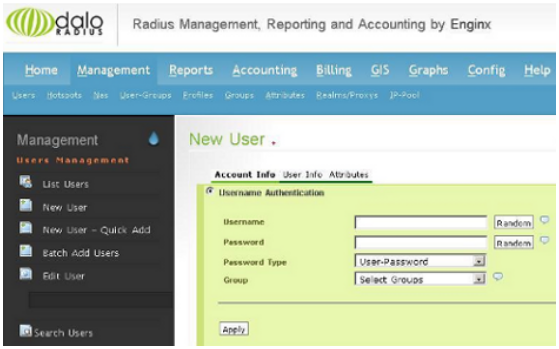
\includegraphics[width=0.75\linewidth]{./3_Tecnologias/Img/daloRADIUS1.png}
\end{center}
\caption{Pantalla de adición de nuevo usuario}
\label{daloRADIUS1}
\end{figure}

\subsection{CoovaChilli}
CoovaChilli es un \emph{software} controlador de acceso WiFi a Internet de código abierto basado en el antiguo proyecto ChilliSpot, ya abandonado. Lanzado bajo \emph{GNU General Public License} (GPL), en la actualidad es mantenido por los aportes de personal original de ChilliSpot. CoovaChilli carece de interfaz gráfica, por lo que ha de controlarse utilizando la orden chilli en el terminal. Proporciona un entorno de portal cautivo y utiliza RADIUS o \emph{Hyper Text Transfer Protocol} (\acrshort{HTTP}) para proporcionar acceso y contabilidad. CoovaChilli es parte integral de CoovaAP, un firmware basado en OpenWRT especializado en \emph{hotspots}. Soporta dos métodos de acceso diferentes para una red local inalámbrica: \emph{Universal Access Method} (\acrshort{UAM}) y WPA.

\subsubsection{Funcionamiento}
Utiliza mediante tres interfaces principales:

\begin{itemize}
\item De enlace descendente (\emph{downlink}) que acepta conexiones de los clientes, mediante DHCP y ARP. Los clientes pueden encontrarse en dos estados: no autenticados y autenticadas. En este último caso, sus peticiones Web son redirigidas a un portal cautivo, el servidor Web de autenticación que usualmente les solicita usuario y contraseña. El servidor Web envía las credenciales del usuario al proceso chilli mediante redirecciones del navegador.  
\item De RADIUS para autenticar a los clientes. Para el método de acceso UAM se utilizan desafíos y contraseñas CHAP de acuerdo a la RFC 2865. Para la autenticación por WPA se utiliza el atributo de mensaje EAP para RADIUS de acuerdo a la RFC 2869. Los atributos de mensaje descritos en la RFC 2548 se usan para transferir claves de cifrado desde el servidor RADIUS hacia CoovaChilli. Si la autenticación tiene éxito el estado del cliente pasa a ser de autenticado. 
\item De enlace ascendente (\emph{uplink}) para dirigir el tráfico hacia otras redes. 
\end{itemize}

La interfaz de enlace ascendente se implementa utilizando drivers \emph{network tunnel} (\acrshort{TUN}) que opera con el encaminamiento de datagramas IP y network \acrshort{TAP} que opera a nivel de puente (\emph{bridge}) con datagramas de nivel de enlace (normalmente Ethernet). TUN/TAP funcionan como dispositivos de comunicación virtuales del núcleo del sistema operativo encargados de recoger datos del nivel de aplicación y enviarlos a la Red y viceversa. Cuando el proceso \emph{chilli} comienza se habilita una interfaz TUN y se llama a un \emph{script} de configuración externo opcional. Esto es, las interfaces TUN/TAP son interfaces \emph{software}, solo existen en el núcleo del sistema y se utilizan para realizar funciones de red a nivel de espacio de usuario. Una vez implantadas actúan como cualquier otra interfaz del sistema. Se les pueden asignar direcciones IP, su tráfico puede ser analizado, se puede determinar qué caminos le apuntan, añadirles directivas de cortafuegos...

\subsubsection{Configuración}

El archivo principal de CoovaChilli es  \emph{/usr/local/etc/chilli.conf} el cual incluye otros tres: \emph{main.conf}, \emph{hs.conf} y \emph{local.conf}. Los dos primeros son creados por los scripts del shell existentes en el archivo \emph{functions} basándose en las configuraciones de otros archivos mencionados a continuación y obteniendo algunas configuraciones del servidor RADIUS y otras \acrshort{URL}. El archivo \emph{local.conf} está reservado para configuraciones de lugares específicos.
Las configuraciones por defecto que son establecidas en \emph{chilli.conf} se encuentran en \emph{/usr/local/etc/chilli/defaults}. Los valores existentes en este último archivo pueden sobreescribirse durante la inicialización de chilli si existe otro archivo en \emph{/usr/local/etc/chilli/config}, que no es más que una copia del archivo defaults sobrescribiendo los valores de los atributos que se desea cambiar.
Cada vez que se enciende el dispositivo en el que está instalado CoovaChilli, el script presente en \emph{/usr/local/etc/init.d/chilli} se ejecuta tomando las configuraciones de los archivos \emph{defaults} y \emph{config} mencionados anteriormente, ejecutando también el script \emph{/usr/local/etc/chilli/functions} para asistir en esta configuración y la de otros archivos relevantes para el funcionamiento del programa, creando de este modo los respectivos archivos \emph{main.conf}, \emph{hs.conf} y \emph{local.conf}.

Adicionalmente, CoovaChilli implementa un servidor Web mínimo destinado a servir contenido en el directorio \emph{/etc/local/etc/chilli/www/}, lugar en el que puede ubicarse un servicio de portal cautivo sencillo. Por defecto, en este directorio se implementa un portal cautivo con pantalla de espera que redirige a un formulario ensamblado con plantillas HTML y archivos de Web scripts \emph{Common Gateway Interface} (\acrshort{CGI}) para contenido dinámico. Estos archivos (con la extensión .chi) son procesados con el software Haserl \cite{Haserl}, por lo que si se usa la configuración por defecto de CoovaChilli este programa ha de estar instalado.

Aunque CoovaChilli cuenta con numerosas opciones, en este TFG se usa y modifica tan solo un subconjunto de ellas, asignándoles valores en los archivos \emph{defaults} y \emph{config}:

\begin{itemize}
\item \emph{HS\_WANIF}: especifica la interfaz de red que cuenta con acceso a internet, habitualmente la interfaz Ethernet del dispositivo, \emph{eth0}.
\item \emph{HS\_LANIF}: interfaz a la que se conectan los clientes, habitualmente la interfaz WiFi del dispositivo, \emph{wlan0}.
\item \emph{HS\_NETWORK}: dirección IP de la red a la que se conectan los clientes, por ejemplo 192.160.10.0. Habitualmente esta dirección es la determinada al configurar una IP estática para \emph{wlan0} en el archivo \emph{/etc/network/interfaces} del sistema operativo.
\item \emph{HS\_UAMLISTEN}: la IP del dispositivo de red al que se conectan los clientes. Por supuesto, debe pertenecer al rango IP de la red especificada en el atributo anterior, siguiendo el ejemplo dicha IP sería 192.168.10.1.
\item \emph{HS\_UAMALLOW}: redes y dominios en los que los usuarios no autenticados sí tienen permitida la navegación. Habitualmente solo se permite la red local desde la que también se serviría el portal cautivo (el mismo valor que el atributo \emph{HS\_NETWORK}), aunque para otros servicios de portal cautivo más avanzados podría permitirse el acceso a otros dominios, por ejemplo a la URL de la correspondiente API de Facebook para la autenticación por esta red social o al dominio de PayPal para realizar pagos de tarifas.
\item \emph{HS\_UAMSECRET}: clave secreta con la que se cifran las credenciales que se envíen desde el servidor Web del portal cautivo hacia CoovaChilli.
\item \emph{HS\_UAMFORMAT}: ubicación y puerto del servidor Web que proporcionaría el portal cautivo.
\item \emph{HS\_UAMHOMEPAGE}: ubicación y puerto a la que se redirigirían las peticiones Web de los clientes al conectarse a la red. Habitualmente, esto es una página de bienvenida que luego redirige hacia el contenido servido en la ubicación especificada en \emph{HS\_UAMFORMAT}.
\item \emph{HS\_SSID}: SSID de la red.
\end{itemize}

\subsubsection{Interfaz \emph{JavaScript Object Notation}}

\emph{JavaScript Object Notation} (JSON) es perfil de transmición de datos desde un servidor Web a un navegador. Tiene menos datos de cabecera que el \emph{Xtensible Markup Language} (\acrshort{XML}) habitualmente utilizado en \emph{Asynchronous JavaScript And XML}(\acrshort{AJAX}) y otros servicios y por ello se ha considerado una alternativa a este y ha alcanzado gran popularidad. CoovaChilli usa JSON para realizar el control de usuarios de forma que pueda utilizarse un portal cautivo de cualquier tipo e incluso en servidores distintos al incorporado en el programa a los que pueda acceder el cliente, previa habilitación del acceso al dominio correspondiente en el atributo \emph{HS\_UAMALLOW} del archivo de configuración. Un usuario puede autenticarse a través de ella, obtener el estado de su conexión o desconectarse del portal cautivo.

Para comunicarse con la interfaz JSON de CoovaChilli se utiliza una biblioteca JavaScript, instalada por defecto en \emph{/usr/local/etc/chilli/www/ChilliLibrary.js}. Esta biblioteca crea el objeto global \emph{chilliController}, que ha de inicializarse con los valores necesarios según nuestra configuración. El portal cautivo que se implemente pasa a utilizar los métodos expuestos por el objeto \emph{chilliController} para comunicarse con CoovaChilli, enviándole peticiones HTTP GET a este y recibiendo respuestas en el formato JSON.

El objeto \emph{chilliController} puede enviar los siguientes órdenes a CoovaChilli:

\begin{itemize}
\item \emph{logon}: intenta un login utilizando CHAP. La respuesta contendría los datos de sesión y los datos iniciales de contabilidad. Es llamado mediante el método \emph{logon(username, password)}.
\item \emph{logoff}: termina la sesión actual. Es llamado mediante el método \emph{logoff()}.
\item \emph{status}: proporciona los datos de contabilidad más recientes. Es llamado mediante el método \emph{refresh()}.
\end{itemize}

\begin{listing}[H]
\begin{minted}
[
frame=lines,
framesep=2mm,
baselinestretch=1.2,
bgcolor=lightgray,
fontsize=\footnotesize,
breaklines=true,
breaksymbolleft={}
]
{html}
<script src="http://my.host.com/ChilliLibrary.js"></script>
<script> 
  chilliController.host = "10.0.0.1";
  chilliController.port  = 4003;
  chilliController.interval = 60;

  chilliController.onError  = handleErrors;
  chilliController.onUpdate = updateUI ;

  function updateUI( cmd ) {
    alert ( 'You called the method' + cmd +
      '\n Your current state is =' + chilliController.clientState ) ;
  }
  
  function handleErrors ( code ) {
    alert ( 'The last contact with the Controller failed. Error code =' + code );
  }

  chilliController.refresh();
</script>
\end{minted}
\caption{Plantilla de código de CoovaChilli para el manejo de la interfaz JSON}
\label{JSONTemplate}
\end{listing}

Cuando un cliente es autorizado, el objeto \emph{chilliController} consulta periódicamente la información de contabilidad, enviando órdenes de \emph{status} para actualizar los datos (orden \emph{autorefresh}).
CoovaChilli facilita una plantilla de código en su página Web que puede alojarse en el HTML de un portal cautivo que utilice esta interfaz (Bloque de código \ref{JSONTemplate}).

El \emph{chilliController} es un objeto global creado por el script incluido al principio. Por defecto, está configurado para contactar con CoovaChilli en 192.168.182.1:3990 cada 30 segundos. Si deseamos valores diferentes, pueden modificarse antes de llamar a cualquier método tal y como se ve en el bloque de código. Tras configurar el objeto \emph{chilliController} se debe llamar al método \emph{refresh()} para determinar el estado actual del cliente.

CoovaChilli ha implementado los siguientes atributos para el objeto ChilliController. Al ser una interfaz que continúa expandiéndose y desarrollándose existen otros atributos aún no implementados pero presentes en la documentación que se han omitido en este TFG.

\begin{itemize}
\item \emph{host}: la dirección IP del controlador de acceso de CoovaChilli.
\item \emph{port}: el puerto HTTP para las peticiones JSON.
\item \emph{interval}: intervalo medido en segundos. Mientras el usuario está autenticado, los datos de contabilidad y de sesión se actualizan mediante \emph{polling} a CoovaChilli a este intervalo.
\item \emph{language}: el idioma preferido para el mensaje de respuesta (código de idioma de dos letras ISO, por ejemplo ‘en’).
\item \emph{clientState}: estado del terminal. \emph{UNKNOWN} significa que aún no se ha recibido información desde CoovaChilli. Otros valores posibles son \emph{NOT\_AUTHORIZED}, \emph{AUTHORIZED} y \emph{AUTH\_PENDING}.
\item \emph{command}: el último comando enviado a CoovaChilli (que podría estar pendiente): \emph{logon, logoff, refresh, autorefresh}.
\item \emph{sessionId}: identificador único de sesión generado por CoovaChilli (\emph{Acct-Session-Id}). Se utiliza para asegurar que las propiedades del miembro de la sesión y el miembro de la contabilidad pertenezcan a la misma sesión.
\item \emph{message}: mensaje a ser mostrado al usuario. Puede ser el Mensaje Respuesta RADIUS o un mensaje generado por CoovaChilli.
\item \emph{redir}: este atributo expone datos leídos en la URL de la redirección inicial que se realiza hacia el portal cautivo indicado en el atributo de configuración de \emph{HS\_UAMHOMEPAGE}. Solo existe si la página especificada en dicho atributo incluye un script manejador de \emph{chilliController}.
\item \emph{originalURL}: URL pedida originalmente por el cliente antes de su redirección.
\item \emph{redirectionURL}: URL a la que se va a redirigir a continuación.
\item \emph{macAddress}: atributo RADIUS \emph{Calling-Station-Id}. La dirección MAC del dispositivo cliente.
\item \emph{ipAddress}: atributo RADIUS \emph{Framed-IP-Address}.
\item \emph{location}: este atributo contiene información básica sobre la ubicación.
\item \emph{name}: atributo RADIUS \emph{WISPr-Location-Name}, el nombre de la ubicación también almacenada en el atributo locationname o radiuslocationname de chilli.conf.
\item \emph{session}: expone los atributos RADIUS recibidos en el paquete RADIUS \emph{access-attempt}. Estos atributos son fijos durante una sesión.
\item \emph{startTime}: el momento de inicio de sesión de CoovaChilli. Es un objeto Date de ECMAScript. No es un atributo RADIUS.
\item \emph{sessionTimeout}: temporizador para la finalización de sesión.
\item \emph{idleTimeout}: temporizador para el tiempo de inactividad.
\item \emph{accounting}: valores de contabilidad de Volumen/Tiempo. Van cambiando durante la sesión.
\item \emph{sessionTime}: atributo RADIUS \emph{Acct-Session-Time}. La duración de la sesión.
\item \emph{idleTime}: tiempo de inactividad calculado por CoovaChilli (el tráfico desde o hacia CoovaChilli es ignorado). No es un atributo RADIUS, pero el objeto controlador lo utiliza para planificar la siguiente actualización de datos tras una desconexión por IdleTimeout.
\item \emph{inputOctets}: atributo RADIUS \emph{Acct-Input-Octets}.
\item \emph{outputOctets}: atributo RADIUS \emph{Acct-Output-Octets}.
\item \emph{inputGigawords}: atributo RADIUS \emph{Acct-Input-Gigawords}.
\item \emph{outputGigawords}: atributo RADIUS \emph{Acct-Output-Gigawords}.
\end{itemize}

CoovaChilli ha implementado los siguientes manejadores de eventos:

\begin{itemize}
\item \emph{onUpdate}: función llamada cuando el objeto chilliController se actualiza. Las actualizaciones ocurren cuando nuevos datos se reciben desde el controlador. Esto puede ocurrir después de que un método se llame explícitamente (\emph{logon, logoff, refresh}) o automáticamente a intervalos determinados por el atributo interval, cuando se autoriza al cliente (\emph{autorefresh}). La función recibe el nombre de la orden que causó la actualización como argumento.
\item \emph{onError}: función llamada cuando no puede obtenerse una respuesta JSON correcta del controlador (se ha caído el enlace inalámbrico, la sintaxis JSON es incorrecta…). La función recibe un código de error como argumento.
\end{itemize}

Como se ha mencionado anteriormente, los órdenes se envían a CoovaChilli mediante peticiones HTTP. El parámetro GET \emph{lang} se usa en \emph{logon} para pasar el idioma preferido. El campo \emph{version} se utiliza para controlar las diferentes versiones del protocolo JSON de CoovaChilli. Si un parámetro para hacer \emph{callbacks} existe, CoovaChilli pone el texto de salida JSON entre paréntesis y lo adjunta con la función de \emph{callback}. La salida sería como una llamada a una función con el objeto JSON pasado como parámetro.

Para el logon, siguiendo el ejemplo del bloque de código que configuró el objeto \emph{chilliController} en apartados anteriores, cuando se llama al método \emph{logon()} del Controlador el objeto genera un desafío CHAP aleatorio (\emph{string} hexadecimal) y realiza la petición a la \acrshort{URL} \emph{http://192.168.182.1:3990/json/logon} con las siguientes \emph{strings} de petición: \emph{?username=XXXX\&chapchallenge=YYYY\&chappassword=0123456789abcdef\&lang=EN}.
CoovaChilli responde con un objeto en formato JSON del bloque de código \ref{JSONResponseYES}:

\begin{listing}[H]
\begin{minted}
[
frame=lines,
framesep=2mm,
baselinestretch=1.2,
bgcolor=lightgray,
fontsize=\footnotesize,
breaklines=true,
breaksymbolleft={}
]
{json}
{
  "version" : "1.0",
  "clientState" : 1 ,
  "sessionId" : "4662e92b0000000e" ,
  "message" : "You're now connected" ,
  "location" : {
     "name":  "Coova labs"
  },
 
  "redir" : {
    "macAddress" : "00-30-1B-B5-03-6B",
    "originalURL" : "http://my.yahoo.com/",
    "redirectionURL" : "http://www.coova.org/welcome.php",
    "ipAddress" : "192.168.182.47"
  },
 
  "session" : {
    "startTime" : 137550720,
    "terminateTime" : 13756072,
    "sessionTimeout" : 3600,
    "idleTimeout" : 240,
    "maxInputOctets" : 100000000,
    "maxOutputOctets" : 100000000,
    "maxTotalOctets" : 100000000,
    "bandwidthMaxDown" : 1000000,
    "bandwidthMaxUp" : 1000000
  },
  
  "accounting": {
     "sessionTime" : 2,
     "idleTime" : 0,
     "inputOctets" : 0,
     "outputOctets" : 0,
     "inputGigawords" : 0,
     "outputGigawords" : 0
  }
}
\end{minted}
\caption{Respuesta de la interfaz JSON a un logon()}
\label{JSONResponseYES}
\end{listing}

Si por el contrario la autorización no tiene éxito la respuesta JSON será la que se muestra en el bloque de código \ref{JSONResponseNO}.

\begin{listing}[H]
\begin{minted}
[
frame=lines,
framesep=2mm,
baselinestretch=1.2,
bgcolor=lightgray,
fontsize=\footnotesize,
breaklines=true,
breaksymbolleft={}
]
{json}
{
  "version": "1.0",
  "clientState": 0,
  "message": "This username does not exist",
  "location" : { "name":"My HotSpot" }
 }
\end{minted}
\caption{Respuesta de la interfaz JSON a un logon() fallido}
\label{JSONResponseNO}
\end{listing}

Para el \emph{logoff}, cuando se llama al método de desconexión se realiza la petición a \emph{http://192.168.182.1:3990/json/logoff?lang=en\&callback=myfunc}. La respuesta JSON pasa a tener esta forma: \emph{myfunc (\{``version'': ``1.0'', ``clientState'': 0\})}.

Para el \emph{Refresh}, cuando se llama al método de actualización se realiza la petición a \emph{http://192.168.182.1:3990/json/status?lang=en}. La respuesta JSON en este caso se muestra en el bloque de código \ref{JSONRefresh1}.

\begin{listing}[H]
\begin{minted}
[
frame=lines,
framesep=2mm,
baselinestretch=1.2,
bgcolor=lightgray,
fontsize=\footnotesize,
breaklines=true,
breaksymbolleft={}
]
{json}
{
 "version" : "1.0",
 "clientState" : 1 ,
 "sessionId" : "4662e92b0000000e" ,
 "accounting": {
     "sessionTime" : 1230,
     "idleTime" : 240,
     "inputOctets" : 2912981 ,
     "outputOctets" : 51498511,
     "inputGigawords" : 0,
     "outputGigawords" : 0
  }
}
\end{minted}
\caption{Respuesta de la interfaz JSON a un refresh()}
\label{JSONRefresh1}
\end{listing}

No es necesario repetir las propiedades fijas de sesión. El atributo \emph{sessionId} se usa para asociar los nuevos valores de contabilidad recibidos con los valores de sesión recibidos con la orden \emph{logon} inicial.

Si el cliente no está autorizado se envía esta respuesta a las peticiones la respuesta sería la del bloque de código \ref{JSONNoAuthorized}.

\begin{listing}[H]
\begin{minted}
[
frame=lines,
framesep=2mm,
baselinestretch=1.2,
bgcolor=lightgray,
fontsize=\footnotesize,
breaklines=true,
breaksymbolleft={}
]
{json}
{
 "version" : "1.0",
 "clientState" : 0
}
\end{minted}
\caption{Respuesta de la interfaz JSON a una petición no autorizada}
\label{JSONNoAuthorized}
\end{listing}

\subsection{El entorno node.js para programación de back-end}

JavaScript junto a HTML y CSS son los tres pilares básicos de la programación \emph{front-end} (cliente). Los servidores (\emph{back-end}), suelen estar programados en otros lenguajes como \emph{Hypertext Preprocessor} (PHP), Java \cite{JavaServer} o Python \cite{Python}... Poco a poco JavaScript se ha convertido en una opción para programar los \emph{back-ends} debido a la aparición de Node.js.  Esto se debe a la iniciativa de intentar unificar todo el desarrollo Web en un único lenguaje de programación introduciendo el  paradigma \emph{JavaScript en todas partes}.

El Node.js tiene una arquitectura dirigida por eventos capaz de manejar la entrada-salida asíncrona, en un esfuerzo por aumentar la escalabilidad y la tasa de transmisión en aplicaciones Web con gran cantidad de operaciones de este tipo o aplicaciones Web en tiempo real. Su funcionalidad se basa en bibliotecas JavaScript conectadas entre ellas y al sistema operativo por medio de \emph{bindings} en C++. Utiliza una combinación del motor JavaScript V8 de Google \cite{V8}, un bucle de eventos y una API de entrada-salida de bajo nivel. El motor V8 fue desarrollado para Google Chrome, escrito en el lenguaje C++. Se encarga de compilar el código JavaScript a código máquina nativo en lugar de interpretarlo en tiempo real. El bucle de eventos se implementa en un único hilo de ejecución que atiende llamadas de entrada-salida no bloqueantes, permitiendo un número elevado de conexiones concurrentes sin incurrir en los costes de recursos del cambio de contexto entre hilos. Mediante el patrón de diseño software \emph{observador}, cada función que realice una operación de entrada-salida debe usar un \emph{callback}, una función pasada como parámetro que se ejecuta al terminar dicha operación.

Con Node.js es muy sencillo implantar un servidor Web básico que responda a cualquier petición utilizando tan solo una de sus funcionalidades incluidas, el paquete HTTP, tal como se muestra en el código del bloque de código \ref{NodeServer}.


\begin{listing}[H]
\begin{minted}
[
frame=lines,
framesep=2mm,
baselinestretch=1.2,
bgcolor=lightgray,
fontsize=\footnotesize,
breaklines=true,
breaksymbolleft={}
]
{javascript}
// Load HTTP module
var http = require("http");

// Create HTTP server and listen on port 8000 for requests
http.createServer(function(request, response) {

   // Set the response HTTP header with HTTP status and Content type
   response.writeHead(200, {'Content-Type': 'text/plain'});
   
   // Send the response body "Hello World"
   response.end('Hello World\n');
}).listen(8000);

// Print URL for accessing server
console.log('Server running at http://127.0.0.1:8000/');
\end{minted}
\caption{Implementando un servidor web con Node.js}
\label{NodeServer}
\end{listing}

Este sencillo código, al ejecutarse en Node.js, implementa una respuesta de texto plano \emph{Hello World} al recibir cualquier petición HTTP en la dirección IP de \emph{loopback} del sistema, 127.0.0.1 en IPv4, y el puerto 8000.

\subsubsection{El gestor de paquetes npm}

Como parte del entorno de Node.js se incluye \emph{npm}, un gestor de paquetes JavaScript utilizado para instalar bibliotecas adicionales almacenadas en el registro npm, un repositorio online de paquetes públicos. 
Permite tanto instalar como distribuir módulos y gestionar las dependencias de un proyecto determinado desde la línea de órdenes, dependencias que luego pueden utilizarse en el proyecto mediante el método \emph{require()}. 
Puede gestionar paquetes JavaScript instalados globalmente. Mediante un archivo \emph{package.json} ubicado habitualmente en la raíz de un proyecto Node.js, \emph{npm} puede instalar todas las dependencias necesarias con una sola orden, atendiendo al rango de versiones posibles para evitar incompatibilidades.

\subsubsection{El \emph{framework Express}}
Express, también referido como \emph{Express.js}, es un \emph{framework} para Node.js. Instalable mediante \emph{npm}, está diseñado para desarrollar tanto aplicaciones Web como API y se ha convertido en el \emph{framework} de servidor estándar de facto para Node.js. Intenta ser mínimo a la par que flexible, pudiendo implantar un servidor sencillo en unas pocas líneas de código e ir implementando las funcionalidades requeridas según sea necesario.

Express representa parte del \emph{back-end} de lo que se ha dado a conocer como el \emph{\acrshort{MEAN} stack}, un conjunto de subsistemas de software basados en JavaScript y constituido por \emph{MongoDB} \cite{MongoDB}, un sistema de bases de datos no-SQL, \emph{Angular}, un \emph{framework} para implantar patrones de diseño software de \emph{Modelo-Vista-Controlador} (MVC) en aplicaciones Web de página única, \emph{Express} y el propio Node.js.

Para implantar la funcionalidad del código del ejemplo anterior, esta vez haciendo uso del \emph{framework} Express, puede escribirse el código del bloque de código \ref{ExpressServer} en un archivo JavaScript llamado por ejemplo \emph{app.js} y luego ejecutar este archivo en la línea de órdenes mediante la orden \emph{node app.js}.


\begin{listing}[H]
\begin{minted}
[
frame=lines,
framesep=2mm,
baselinestretch=1.2,
bgcolor=lightgray,
fontsize=\footnotesize,
breaklines=true,
breaksymbolleft={}
]
{javascript}
var express = require('express');
var app = express();

app.get('/', function(req, res) {
  res.send('Hello World!');
});

app.listen(3000, function() {
  console.log('Example app listening on port 3000!');
});
\end{minted}
\caption{Servidor Web implementado con Express}
\label{ExpressServer}
\end{listing}

Las dos primeras líneas realizan la importación del módulo Express y crean la aplicación en la variable \emph{app}, que contendría todos los métodos para recibir las peticiones HTTP, configurar lógicas adicionales y otros controles de comportamiento de la aplicación Web. La orden \emph{app.get()} representa la definición de un camino; especifica una función \emph{callback} como segundo parámetro que se ejecutaría cuando haya una petición HTTP GET con la ruta determinada en el primer parámetro (relativa a la raíz). La función \emph{callback} tiene objetos de petición y respuesta como argumentos y llama al método \emph{send()} en la respuesta para devolver la \emph{string Hello World}. El bloque final inicia el servidor en el puerto 3000 e imprime un \emph{log} en la consola. Si se visita \url{localhost:3000} en el navegador local después de ejecutar este archivo con Node.js se vería la respuesta.

\subsubsection{El módulo \emph{formidable}}
El módulo \emph{formidable} de análisis sintáctico (\emph{parsing}) de datos de tipo formulario, especializado en subida de archivos a servidores, incluyendo subida múltiple. Con el uso de este paquete \emph{npm} es posible gestionar los datos enviados al servidor desde el portal cautivo.
Para poder hacer uso del módulo primero ha de incluirse al archivo que ejecutamos con \emph{node} mediante la orden \emph{require(‘formidable’)}, como también sucedía con \emph{express} y con el resto de módulos. Su API funciona de la siguiente manera:

\begin{itemize}
\item Se crea un objeto formulario entrante y se asocia a una variable con la siguiente asignación \emph{var form = new formidable.IncomingForm()}.
\item Tras esto, pueden especificarse detalles como el directorio en el se suben los archivos con el siguiente código:  \emph{form.uploadDir = ``/ruta/hacia/el/archivo'';}. 
\item Para realizar el parsing de una petición que incluya datos de tipo formulario se usa la siguiente función, donde \emph{request} es la petición entrante: \emph{form.parse(request);}.
\end{itemize}

Los eventos se manejan con la función \emph{on}, que incluye una \emph{string} con el nombre del evento como primer parámetro y una función \emph{callback} como segundo parámetro, a ejecutar cuando dicho evento ocurre. Ejemplos de eventos son ‘\emph{progress}’, ‘\emph{file}’, ‘\emph{error}’ y ‘\emph{end}’. Un ejemplo de manejo de eventos que gestionaría qué ocurre cuando se ha recibido una petición y todos los archivos ya han terminado de llegar al disco se muestra en el bloque de código \ref{ResponseEvent}.

\begin{listing}[H]
\begin{minted}
[
frame=lines,
framesep=2mm,
baselinestretch=1.2,
bgcolor=lightgray,
fontsize=\footnotesize,
breaklines=true,
breaksymbolleft={}
]
{javascript}
form.on('end', function() {
  // Lugar ideal para enviar una respuesta. 
});
\end{minted}
\caption{Función de callback para cuando termina una transferencia}
\label{ResponseEvent}
\end{listing}

\subsubsection{El \emph{middleware Body-Parser}}
Realiza análisis sintáctico los cuerpos de las peticiones entrantes, a cuyos contenidos puede accederse después mediante el atributo \emph{req.body}.
Tras incluirse en el proyecto, por ejemplo bajo la variable \emph{bodyParser}, puede ser llamado desde el objeto \emph{express()} para utilizar sus funciones mediante la orden \emph{use()}. En el bloque de código \ref{bodyparser}. se presenta un ejemplo genérico para habilitar el parsing de JSON y URL-encoded.

\begin{listing}[H]
\begin{minted}
[
frame=lines,
framesep=2mm,
baselinestretch=1.2,
bgcolor=lightgray,
fontsize=\footnotesize,
breaklines=true,
breaksymbolleft={}
]
{javascript}
var express = require('express')
var bodyParser = require('body-parser')

var app = express()

// parse de application/json
app.use(bodyParser.json())

// parse de application/x-www-form-urlencoded
app.use(bodyParser.urlencoded({ extended: true }))

app.use(function (req, res) {
  res.setHeader('Content-Type', 'text/plain')
  res.write('you posted:\n')
  res.end(JSON.stringify(req.body, null, 2))
})
\end{minted}
\caption{Habilitando opciones de parsing}
\label{bodyparser}
\end{listing}


\subsection{Programación del \emph{front-end}}

El \emph{front-end} implica la producción de contenido, apariencia y comportamiento de una página o aplicación Web de forma que el usuario pueda verla e interactuar con ella. En la actualidad las tecnologías usadas para el desarrollo \emph{front-end} se hallan en proceso de cambio y actualización constante, complicado aún más por la aparición en escena de los diferentes dispositivos actuales capaces de acceder a estas aplicaciones Web, con diferentes tamaños de pantalla y distinto grado de soporte de las tecnologías disponibles.

Las herramientas básicas del desarrollo front-end la forman un conjunto de tres tecnologías. HTML, CSS y JavaScript.

\subsubsection{HTML y  CCS}

La última versión de HTML es conocida como HTML5 y fue publicada en octubre de 2014. Esta versión contiene nuevas formas de manejar elementos, sobre todo en el ámbito de la multimedia (como el audio y el vídeo), y nuevos descriptores y posibilidades de metadatos con los que se busca conseguir una mayor interoperabilidad entre sistemas y una mayor semántica de la Web. Dado que introduce varias API y marcado para aplicaciones Web complejas y también ha sido diseñado teniendo en mente dispositivos de bajo consumo, su uso también está planteado para aplicaciones móviles multiplataforma.

El CSS define el aspecto o la presentación de la página Web. Un documento CSS consiste en listar unas reglas de visualización —color, tipografía, fondo, bordes— para cada elemento de marcado usado después en HTML. De esta forma, CSS trata de separar el contenido y la presentación del mismo, de forma que si se quiere cambiar el diseño gráfico de un sitio Web no haya que modificar todos y cada uno de los documentos HTML existentes, sino un número mucho más reducido de documentos CSS que estén referidos en estos.

Al mismo tiempo, la variedad de módulos existentes actualmente trata de dar un mayor dinamismo y responsividad a las páginas Web, incluyendo animaciones o diseño en múltiples columnas que se adaptan a los tamaños de pantalla.

\subsubsection{JavaScript: bibliotecas, API y complementos}

JavaScript es un lenguaje de programación interpretado de alto nivel que define el comportamiento de una aplicación o página Web (interactividad y ejecución de programas online). Todos los navegadores modernos soportan una implementación parcial o completa de la especificación ECMAScript \cite{ECMAScript2016}.

El \emph{Document Object Module} (\acrshort{DOM}) es la especificación de la jerarquía de los elementos usados por HTML, que puede entenderse como un diagrama de árbol en el que cada objeto representa una parte del documento. JavaScript manipula el DOM pudiendo acceder a cada elemento y realizando cambios en él que luego se verían reflejados en la visualización del sitio Web, a efectos creando HTML dinámico en el que pueden alterarse los elementos y atributos, cambiar el estilo CSS, reaccionar a eventos de la página o crear eventos nuevos. En la Figura \ref{DOMModel} se muestra un ejemplo gráfico del DOM.

\begin{figure}[!t]
\begin{center}
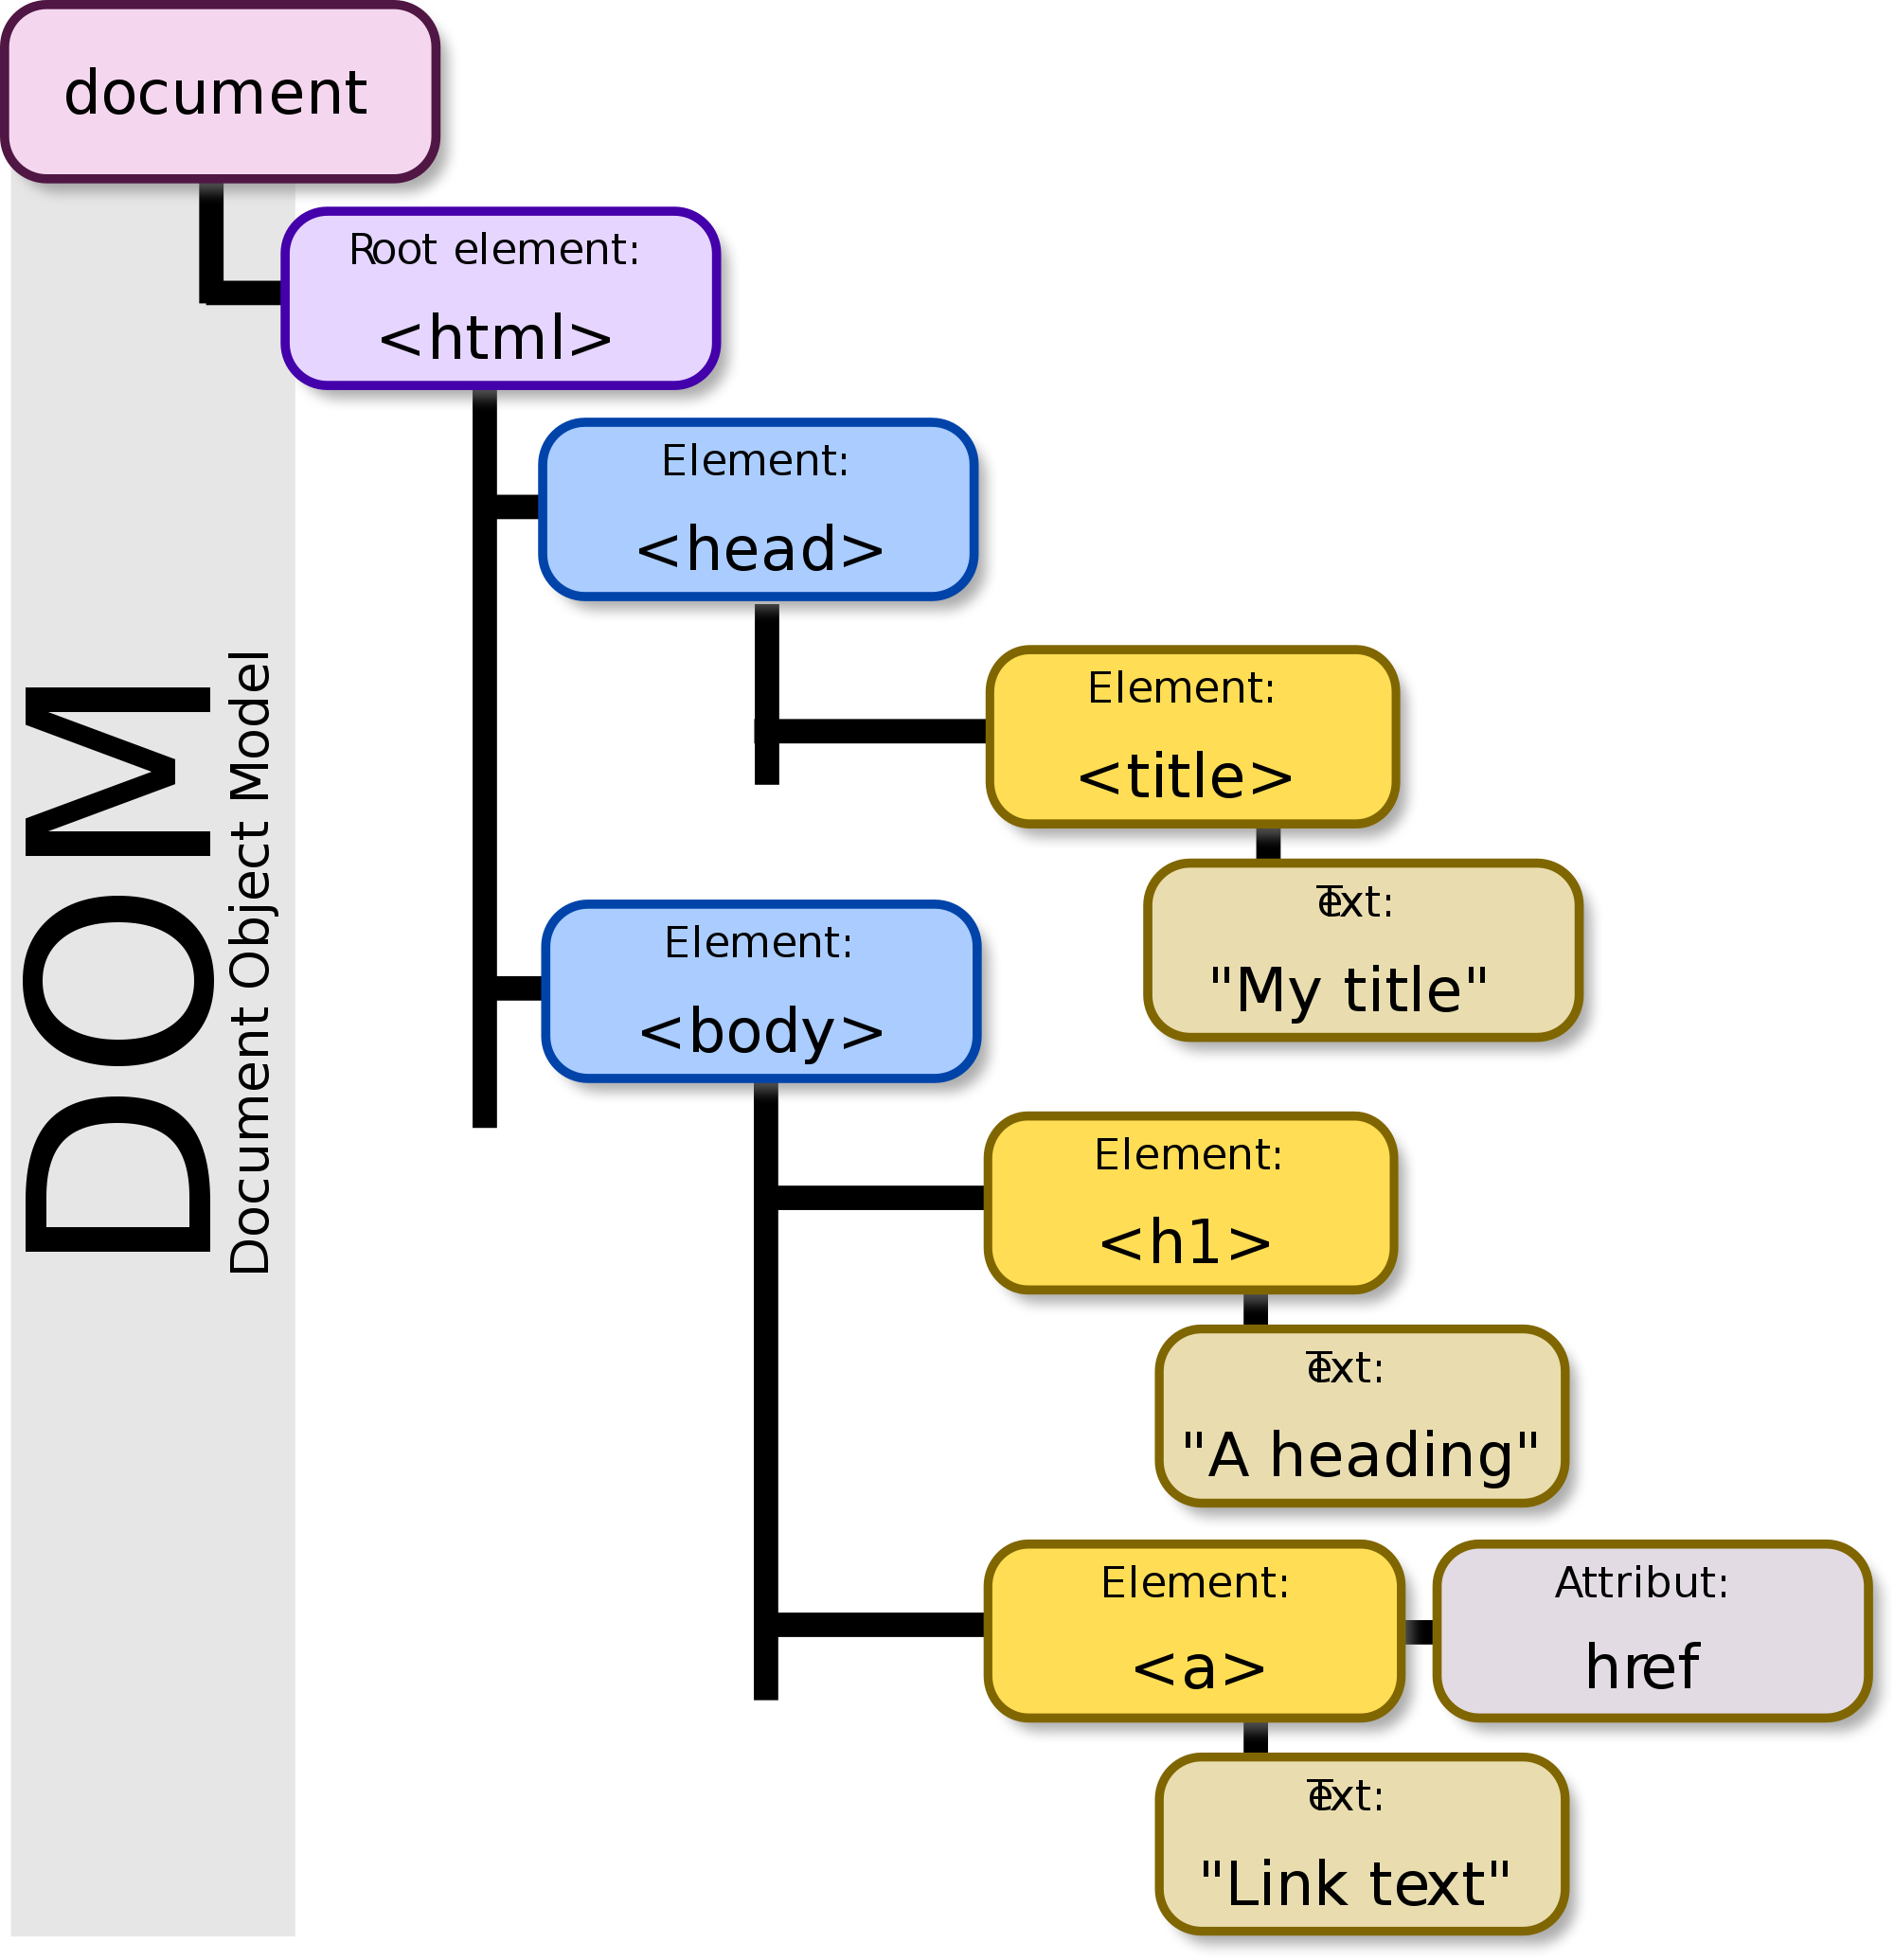
\includegraphics[width=0.75\linewidth]{./3_Tecnologias/Img/DOMModel.png}
\end{center}
\caption{Esquema general del DOM}
\source{https://en.wikipedia.org/wiki/Document\_Object\_Model}
\label{DOMModel}
\end{figure}

Aunque en este TFG se trabaja con el estándar de JavaScript llamado ECMAScript 2016, en la actualidad la última versión es ECMAScript 2017, lanzada en Junio de este mismo año. A continuación se detallan algunos elementos de importancia que se utilizaron en la elaboración de este TFG. Su lugar de uso se detalla en el siguiente capítulo del presente documento.

\paragraph{\emph{Web Real-Time Communications}}~\\

WebRTC es una tecnología que permite a las aplicaciones Web capturar y transmitir datos de audio y vídeo, así como intercambiar datos entre navegadores sin un intermediario. Los estándares que componen WebRTC hacen posible compartir datos y realizar videoconferencias \emph{peer-to-peer}, sin que sea necesario que los usuarios instalen complementos u otros elementos \emph{software} de terceros. Junto a las API \emph{MediaStream Recording} y \emph{Media Capture and Streams} proporcionan a la Web una gama de capacidades multimedia que incluyen captura y grabación de multimedia en disco, conferencias de audio y vídeo, intercambio de archivos e incluso gestión de identidad.

Es un estándar actualmente en desarrollo por la \emph{World Wide Web Consortium} (\acrshort{W3C}) y el IETF. Para transferir los datos multimedia se utiliza el protocolo \emph{Realtime Transport Protocol }(\acrshort{RTP}).

El \emph{getUserMedia()} es el método principal mediante el que se solicitan al usuario los permisos necesarios para usar un dispositivo de entrada multimedia (como la cámara o el micrófono). Produce una interfaz \emph{MediaStream} consistente en las pistas de los tipos de multimedia solicitados. Generalmente se usa accediendo a la interfaz \emph{MediaDevices} con la siguiente orden \emph{navigator.mediaDevices.getUserMedia(constraints).then(...)} siendo \emph{constraints} el parámetro que indica el tipo de multimedia que se solicita y then la función que contendría los callbacks a ejecutar en caso de éxito o error según la \emph{Promise API}.

La API \emph{MediaStream Recording} está muy relacionada captura los datos generados por el objeto \emph{MediaStream} para su análisis, procesado o guardado en disco. Se basa en una única interfaz, \emph{MediaRecorder}, que se encarga de obtener los datos del \emph{MediaStream} mediante una serie de eventos. El proceso de grabación es muy sencillo:

\begin{itemize}
\item Se crea el \emph{MediaStream} fuente de los datos multimedia.
\item Se crea el objeto \emph{MediaRecorder}, especificando la transmisión de origen y otras opciones pertinentes.
\item Configurar el gestor \emph{MediaRecorder.ondataavailable} para el evento \emph{dataavailable}, que sería llamado cada vez que haya datos disponibles.
\item Controlar el proceso de grabación mediante los métodos disponibles, por ejemplo con \emph{MediaRecorder.start()} para comenzar y \emph{MediaRecorder.stop()} para detener la grabación.
\item El evento \emph{dataavailable} tiene un atributo \emph{data} que contiene la información multimedia adquirida, pudiendo procesarse como se requiera.
\end{itemize}

La transmisión de datos en Web puede verse enormemente beneficiada por JSON soportado de forma nativa desde ECMAScript 5, aunque debido a su popularidad son ya muchos los lenguajes que han incluido generadores y analizadores de su sintaxis.

\paragraph{\emph{AJAX}}~\\

AJAX utiliza peticiones HTTP para que las aplicaciones Web puedan enviar datos al servidor y recibir datos del mismo en segundo plano, sin interferir en el comportamiento y la visualización de la Web. De este modo, junto a la manipulación del DOM realizada por JavaScript, se permite cambiar el contenido dinámicamente con información procedente del servidor sin tener que actualizar la totalidad de la página. En la actualidad se utiliza JSON en lugar de XML por su integración nativa con JavaScript.

\paragraph{\emph{jQuery}}~\\

A menudo, trabajar con determinadas funciones de JavaScript (manipulación del DOM, manejar eventos, usar AJAX) puede generar documentos difíciles de leer por su extensión y lo confuso de su sintaxis. La jQuery es una biblioteca JavaScript gratuita y de código abierto que trata de simplificar todos estos procesos del lado del cliente. Permite a los desarrolladores crear complementos con los que añadir una capa más de abstracción a las interacciones de bajo nivel siguiendo un enfoque modular. Actualmente se halla en su versión 3. Para utilizarlo en un sitio Web ha de ser incluido como se incluiría un archivo JavaScript cualquiera en un archivo HTML. La popularidad de jQuery radica en cómo simplifica la lectura y el análisis del código. Por ejemplo, si desde un archivo JavaScript deseamos realizar una petición AJAX de tipo GET al archivo del servidor \emph{send-ajax.php} se tendría que escribir el bloque de código \ref{AJAX} (cliente).

\begin{listing}[H]
\begin{minted}
[
frame=lines,
framesep=2mm,
baselinestretch=1.2,
bgcolor=lightgray,
fontsize=\footnotesize,
breaklines=true,
breaksymbolleft={}
]
{javascript}
// Inicializar la petición HTTP.
var xhr = new XMLHttpRequest();
xhr.open('get', 'send-ajax-data.php');

// Monitorizar los cambios de estado de la petición.
xhr.onreadystatechange = function () {
    var DONE = 4; // readyState = DONE significa que la petición se ha hecho.
    var OK = 200; // status 200 es un retorno con éxito.
    if (xhr.readyState === DONE) {
        if (xhr.status === OK) {
            console.log(xhr.responseText); // Aquí estaría la respuesta del servidor
        } else {
          console.log('Error: ' + xhr.status); // Ha ocurrido un error durante la petición.
        }
    }
};
// Enviar la petición a send-ajax-data.php
xhr.send(null);
\end{minted}
\caption{Petición AJAX normal}
\label{AJAX}
\end{listing}

El mismo ejemplo utilizando jQuery, donde el carácter \$ representa el objeto jQuery a través del cual se accede a todos sus usos, se muestra en el bloque de código \ref{jQueryAJAX}.

\begin{listing}[H]
\begin{minted}
[
frame=lines,
framesep=2mm,
baselinestretch=1.2,
bgcolor=lightgray,
fontsize=\footnotesize,
breaklines=true,
breaksymbolleft={}
]
{javascript}
$.get('send-ajax-data.php')
    .done(function(data) {
        console.log(data);
    })
    .fail(function(data) {
        console.log('Error: ' + data);
    });
\end{minted}
\caption{Petición AJAX con jQuery}
\label{jQueryAJAX}
\end{listing}

\paragraph{\emph{Bootstrap}}~\\

Bootstrap es un \emph{framework} que simplifica la carga de trabajo, adaptada para el diseño de aplicaciones móviles. Contiene plantillas basadas en HTML y CSS para tipografías, formas, botones, navegación y otros componentes, así como algunos componentes opcionales de JavaScript. Utiliza un sistema de rejilla o \emph{grid} para ayudar en el diseño de la web, proporcionando así un sencillo sistema de filas, cada una de ellas subdividida hasta en 12 columnas, con el que puede establecerse la proporción visual de los elementos de la pantalla. En la Figura \ref{gridBootstrap} se muestra un ejemplo de uso del sistema de rejilla en Bootstrap, con un elemento sirviendo de cabecera y varios contenedores alineados bajo el mismo en grupos de tres.

\begin{figure}[!t]
\begin{center}
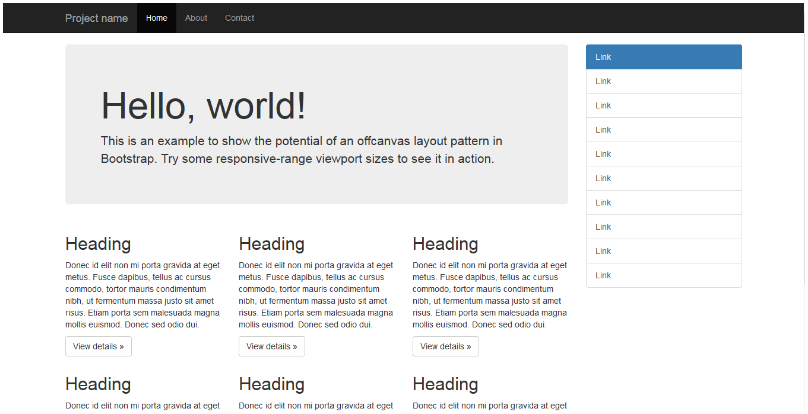
\includegraphics[width=0.75\linewidth]{./3_Tecnologias/Img/gridBootstrap.png}
\end{center}
\caption{Ejemplo de diseño con Bootstrap}
\source{http://getbootstrap.com/docs/4.0/examples/offcanvas/}
\label{gridBootstrap}
\end{figure}